\documentclass[12pt]{article}

%%% Packages
\usepackage[margin=2.5cm]{geometry}
\usepackage{setspace}
\usepackage{lineno}
\usepackage{booktabs}
\usepackage{longtable}
\usepackage{graphicx}
\usepackage{amsmath}
\usepackage{textcomp}
\usepackage[hidelinks]{hyperref}

%%% Graphics path
\graphicspath{{figures/}}

%%% Double spacing and line numbers
\doublespacing
\linenumbers

%%% Begin document
\begin{document}

%% ============================================================
%% TITLE PAGE
%% ============================================================

\begin{titlepage}
\centering
\vspace*{2cm}

{\LARGE\bfseries Inequality in Drug-Susceptible Tuberculosis Quality of Care: A Decomposition and Convergence Analysis Across 195 Countries, 1990--2021\par}

\vspace{2cm}

{\large\textbf{Authors:} [Author list to be finalised]\par}

\vspace{1cm}

{\large\textbf{Correspondence:} [Corresponding author details]\par}

\vspace{1cm}

{\large\textbf{Word count:} \textasciitilde 5900\par}

\vspace{1cm}

{\large\textbf{Keywords:} tuberculosis, health inequality, concentration index, convergence, gender disparity, quality of care, Global Burden of Disease, decomposition analysis\par}

\vfill

\end{titlepage}

%% ============================================================
%% ABSTRACT
%% ============================================================

\section*{Abstract}

\textbf{Background:} Global improvements in drug-susceptible tuberculosis (DS-TB) quality of care have been documented, but the distribution of these gains across countries, sexes, and age groups remains poorly characterised. We quantified inequality in DS-TB care quality using multiple equity metrics and examined whether cross-national disparities are narrowing over time.

\textbf{Methods:} We used a previously developed Quality of Care Index (QCI) for DS-TB, derived from Global Burden of Disease 2021 estimates for 195 countries over 1990--2021. Wealth-related inequality was measured using the Concentration Index (CI) ranked by the Socio-demographic Index (SDI), the Slope Index of Inequality (SII), and the Relative Index of Inequality (RII). Overall dispersion was assessed with the Gini coefficient and Theil index. Wagstaff decomposition identified contributors to the CI. Sigma-convergence (declining cross-country standard deviation) and beta-convergence (faster improvement from lower baselines) were tested using linear regression. Gender disparity was assessed through the female-to-male QCI ratio (GDR) and age-group inequality through within-country QCI range across five age groups.

\textbf{Findings:} The CI was positive throughout the study period, indicating pro-rich concentration, but declined from 0.0121 (95\% CI 0.0091--0.0151) in 1990 to 0.0119 (0.0096--0.0143) in 2021 (linear trend p $<$ 0.001). The Gini coefficient fell by 23.1\% (from 0.0200 to 0.0154) and the Theil T index by 37.8\% (from 0.000714 to 0.000444). Sigma-convergence was confirmed (SD declining at --0.021 points/year, p $<$ 0.001), as was beta-convergence ($\beta$ = --0.377, $R^2$ = 0.345, p $<$ 0.001; half-life 42.2 years). The SII remained stable at approximately 6.8 QCI points (6.73 in 1990, 6.83 in 2021), indicating persistent absolute inequality despite relative convergence. Wagstaff decomposition attributed 40.3\% of the 2021 CI to the mortality-to-incidence ratio, 30.3\% to the YLL-to-YLD ratio, and 29.4\% to the DALY-to-prevalence ratio. Females had higher QCI than males in 97.9\% of countries (mean GDR 1.020 in 2021), with the largest sex gaps in Sub-Saharan Africa (mean gap 2.6 points) and lowest in Europe and Central Asia (1.2 points). The CI was highest for children under 5 years (0.0193) and lowest for children aged 5--14 years (0.0071), indicating that socioeconomic inequality most severely affects care for the youngest. Theil decomposition showed the between-region share of inequality rising from 23.8\% to 34.1\%, suggesting that within-region variation is declining faster than between-region variation.

\textbf{Interpretation:} DS-TB care quality inequality is declining globally but slowly, with a convergence half-life of 42 years. Absolute inequality remains unchanged, and case fatality disparity is the largest contributor to the structural decomposition of the Concentration Index. Targeted investments in low-SDI settings, for males, and for children under 5 are needed to accelerate equity gains toward the 2030 End TB Strategy targets.

\textbf{Funding:} None.

\newpage

%% ============================================================
%% INTRODUCTION
%% ============================================================

\section{Introduction}

Tuberculosis (TB) remains a leading cause of infectious disease mortality, with an estimated 10.6 million incident cases and 1.3 million deaths in 2022.\textsuperscript{1} Despite the availability of effective first-line treatment for drug-susceptible TB (DS-TB), outcomes vary enormously across countries, reflecting disparities in health system capacity, diagnostic access, and broader socioeconomic determinants.\textsuperscript{2,3} The End TB Strategy calls for a 90\% reduction in TB deaths by 2030, but achieving this target requires not only global improvement but equitable distribution of gains across populations.\textsuperscript{4}

We recently developed a composite Quality of Care Index (QCI) for DS-TB using data from the Global Burden of Disease (GBD) Study 2021, which integrates case fatality (mortality-to-incidence ratio), the mortality-to-morbidity balance (YLL-to-YLD ratio), and burden intensity (DALY-to-prevalence ratio) into a single metric scaled 0--100.\textsuperscript{5} The global QCI rose from 91.87 to 95.46 between 1990 and 2021, but substantial cross-national variation persists, with QCI ranging from 82.39 (Afghanistan) to 99.94 (Bermuda) in 2021.

While overall trends have been characterised, the equity dimensions of DS-TB care quality remain unexamined. Several critical questions are unanswered. Is QCI inequality concentrated among wealthier or poorer countries? Is the gap narrowing? Which components of care quality drive inequality most? Do sex and age disparities in QCI vary systematically by development level? Are low-performing countries catching up?

Answering these questions requires formal inequality measurement. The health equity literature offers established tools: the Concentration Index (CI) quantifies wealth-related inequality, the Slope and Relative Indices of Inequality (SII, RII) measure the absolute and relative gradient, and the Gini coefficient and Theil index capture overall dispersion.\textsuperscript{6,7} Decomposition methods can identify determinants of inequality, while convergence analysis tests whether disparities are narrowing.\textsuperscript{8,9}

In this study, we apply a comprehensive suite of inequality and convergence methods to the DS-TB QCI across 195 countries from 1990 to 2021. We decompose the CI to identify which care quality components drive socioeconomic inequality, examine gender and age disparities by region and development level, and test for both sigma- and beta-convergence to assess whether countries are converging toward equal care quality.

%% ============================================================
%% METHODS
%% ============================================================

\section{Methods}

\subsection{Data source and study population}

This study uses the DS-TB Quality of Care Index developed by [Author et al.],\textsuperscript{5} which synthesises GBD 2021 estimates of incidence, prevalence, mortality, DALYs, YLLs, and YLDs for DS-TB into a composite score via principal component analysis. The QCI is available for 204 countries and territories, 31 years (1990--2021), seven age groups, and three sex categories. For inequality analyses, we restricted to 195 countries with both QCI data and SDI values, excluding subnational entities and aggregate regions. Unless otherwise stated, all analyses use age-standardised, both-sexes QCI values.

The Socio-demographic Index (SDI), a composite of per-capita income, educational attainment, and total fertility rate,\textsuperscript{10} served as the socioeconomic ranking variable for wealth-related inequality measures. Country-level SDI values for 2021 were obtained from the GBD.

\subsection{Index scope and component collinearity}

Because the QCI is derived from three GBD-based outcome ratios (MIR, YLLtoYLD, DALtoPER) that share input quantities by construction, the three ratios are mathematically related rather than measurement-independent, and the high proportion of variance captured by PC1 in the source paper (87.98\%) reflects this structural collinearity.\textsuperscript{5} Throughout this study the QCI is therefore interpreted as a smoothed composite of population-level mortality-intensity rather than as a multidimensional measure of orthogonal care-quality domains, and ``Quality of Care'' refers to outcome-based, ecological performance rather than to process-of-care quality. This interpretive framing is important for the inequality analyses that follow, particularly the Wagstaff decomposition (below), in which the regression of QCI on its three components attains $R^2$ near unity by construction; we therefore treat the component-level decomposition as a structural attribution of the index's own variance rather than as the identification of independent causal determinants of inequality.

\subsection{Concentration Index}

The Concentration Index (CI) quantifies the extent to which a health variable is concentrated among advantaged or disadvantaged populations when ranked by a socioeconomic indicator.\textsuperscript{6} We computed the CI using the covariance formula:

\begin{equation}
\text{CI} = \frac{2 \cdot \text{cov}(h_i, R_i)}{\mu}
\end{equation}

where $h_i$ is the QCI for country $i$, $R_i$ is the fractional rank of country $i$ by SDI, and $\mu$ is the mean QCI. A positive CI indicates pro-rich concentration (higher QCI among higher-SDI countries); CI = 0 indicates perfect equality. Standard errors were estimated using the Kakwani approximation.\textsuperscript{11} CIs were computed for each year 1990--2021 to assess temporal trends, and a linear regression of CI on year tested for significant time trends.

Concentration curves were constructed by plotting the cumulative proportion of QCI against the cumulative proportion of countries ranked by SDI, for 1990 and 2021 separately.

\subsection{Slope and Relative Indices of Inequality}

The Slope Index of Inequality (SII) was estimated by regressing QCI on the fractional rank of SDI using ordinary least squares.\textsuperscript{7} The SII represents the absolute difference in QCI predicted between the most and least advantaged countries. The Relative Index of Inequality (RII) was computed as SII divided by the mean QCI, providing a relative measure that accounts for changes in the overall QCI level over time.

\subsection{Gini coefficient and generalised entropy indices}

The Gini coefficient was computed to measure overall dispersion of QCI across countries, irrespective of socioeconomic ranking.\textsuperscript{12} The Theil T index (generalised entropy, $\alpha$ = 1) and the mean log deviation (Theil L, $\alpha$ = 0) were calculated to provide decomposable measures of inequality. The coefficient of variation (CV), standard deviation (SD), and interquartile range (IQR) supplemented these measures.

\subsection{Theil decomposition}

The Theil T index was decomposed into between-region and within-region components using the seven World Bank regions as the grouping variable.\textsuperscript{13} This decomposition quantifies the proportion of total QCI inequality attributable to differences between regional means versus variation within regions.

\subsection{Wagstaff decomposition of the Concentration Index}

The CI was decomposed following the Wagstaff method to identify the contribution of each determinant to socioeconomic inequality in QCI.\textsuperscript{14} QCI was regressed on the three component ratios (MIR, YLLtoYLD, DALtoPER), SDI, and World Bank region dummy variables. For each determinant $k$, the contribution to the CI was calculated as:

\begin{equation}
C_k = \frac{\beta_k \cdot \bar{x}_k}{\mu} \cdot \text{CI}_k
\end{equation}

where $\beta_k$ is the regression coefficient, $\bar{x}_k$ is the mean of determinant $k$, $\mu$ is the mean QCI, and $\text{CI}_k$ is the concentration index of determinant $k$ with respect to SDI. The residual captures inequality not explained by the included determinants.

\subsection{Gender disparity analysis}

The Gender Disparity Ratio (GDR) was defined as female QCI divided by male QCI, with values greater than 1 indicating female advantage. The GDR was computed for each country and year. Cross-country distributions of the GDR were summarised by World Bank region and SDI quintile. The CI was computed separately for females and males to assess whether wealth-related inequality differs by sex. Spearman correlation tested the association between GDR and SDI.

\subsection{Age-group inequality}

For each country and year, the within-country age-group QCI range (maximum minus minimum across five age groups: $<$5, 5--14, 15--49, 50--69, 70+ years) was computed as a measure of age-related inequality. The CI was calculated separately for each age group to determine which ages experience the greatest socioeconomic inequality. Age-group inequality was compared across SDI quintiles and World Bank regions.

\subsection{Convergence analysis}

\textbf{Sigma-convergence} was assessed by testing for a declining cross-country standard deviation of QCI over time using linear regression of SD on year.\textsuperscript{8} A significantly negative slope indicates that countries are becoming more similar.

\textbf{Unconditional beta-convergence} was tested by regressing the change in QCI (2021 minus 1990) on baseline QCI (1990).\textsuperscript{9} A significantly negative coefficient indicates that countries with lower initial QCI improved faster, consistent with catch-up dynamics. The speed of convergence ($\lambda$) and half-life were estimated from the log-linear specification:

\begin{equation}
\ln\!\left(\frac{\text{QCI}_{2021}}{\text{QCI}_{1990}}\right) = \alpha + \beta \cdot \ln(\text{QCI}_{1990}) + \varepsilon
\end{equation}

where $\lambda = -\ln(1 + \beta) / T$ and half-life $= \ln(2) / \lambda$.

\textbf{Conditional beta-convergence} controlled for SDI to test whether convergence operates after accounting for structural development differences.

\subsection{Multilevel regression analysis}

To quantify the independent associations of SDI, sex, and age with QCI while accounting for the nested structure of repeated observations within countries, we fitted multilevel (mixed-effects) linear regression models with country-level random intercepts using restricted maximum likelihood (REML) estimation.

\textbf{Model~1} regressed QCI on SDI and centred calendar year (centred at 2005) using age-standardised, both-sexes data for all countries and years ($n$ = 6{,}240 observations across 195 countries).

\textbf{Model~2} extended the specification to include a binary female indicator and an SDI-by-female interaction term, using age-standardised data for males and females at four time points (1990, 2000, 2010, 2021) to test whether the sex gap in QCI varies by development level.

\textbf{Model~3} regressed QCI on SDI and age group (categorical, with 15--49 years as reference) using 2021 cross-sectional data for five age groups across all countries to quantify age-group effects after controlling for development level.

\subsection{Software and reporting}

All analyses were conducted in Python 3.11 using pandas, NumPy, SciPy, statsmodels, and scikit-learn. This study follows the GATHER guidelines for reporting health estimates and the RECORD guidelines for reporting equity-focused analyses.\textsuperscript{15}

%% ============================================================
%% RESULTS
%% ============================================================

\section{Results}

\subsection{Wealth-related inequality in QCI}

The Concentration Index was positive throughout the study period, confirming that higher QCI is concentrated among countries with higher SDI (Figure~1). The CI was 0.0121 (95\% CI 0.0091--0.0151) in 1990 and 0.0119 (0.0096--0.0143) in 2021, a decline of 0.0002 (1.3\% relative reduction). The CI magnitude is modest, reflecting the compressed range of the QCI (most countries score 90--100); however, this numerical compression belies substantial underlying differences in TB outcomes---the corresponding SII of 6.8 QCI points translates to a threefold difference in case fatality rates between the top and bottom of the SDI distribution. The linear trend in CI was statistically significant (slope --0.000024 per year, p $<$ 0.001), indicating a gradual shift toward less pro-rich concentration. Notably, the CI peaked at 0.0133 around 2000 before declining, coinciding with the height of the HIV/TB epidemic in Sub-Saharan Africa that temporarily widened socioeconomic disparities.

The concentration curve for 2021 lay closer to the line of equality than the 1990 curve across the full distribution, confirming reduced concentration (Figure~3). Both curves lay below the diagonal, indicating pro-rich inequality: the poorest half of countries (ranked by SDI) accounted for less than half of the total QCI.

\subsection{Absolute and relative inequality}

The Slope Index of Inequality remained remarkably stable over three decades: 6.73 QCI points in 1990 and 6.83 in 2021 (Table~1). This indicates that the predicted absolute gap in QCI between the most and least socioeconomically advantaged countries did not narrow despite improvements in all countries. The RII declined marginally from 0.072 to 0.071, reflecting the rise in mean QCI rather than a reduction in the slope.

The persistence of the SII alongside declining CI reveals a critical distinction: while the relative concentration of QCI by SDI diminished slightly, the absolute gradient remained unchanged. Countries at the bottom of the SDI distribution gained in absolute QCI terms, but higher-SDI countries gained similarly, preserving the slope.

\subsection{Overall dispersion}

The Gini coefficient fell by 23.1\%, from 0.0200 in 1990 to 0.0154 in 2021 (Table~1; Figure~2A). The Theil T index declined by 37.8\% (from 0.000714 to 0.000444), and the Theil L index showed a similar trajectory (Figure~2B). The cross-country standard deviation of QCI fell from 3.49 to 2.83 (18.9\% reduction), the coefficient of variation from 0.037 to 0.030 (19.5\% reduction), and the interquartile range from 3.89 to 3.47 (10.8\% reduction). All measures consistently indicate declining overall dispersion, though the pace of reduction decelerated after 2010.

\subsection{Theil decomposition: between versus within regions}

Decomposition of the Theil index into between-region and within-region components revealed a striking structural shift (Figure~8). While total inequality declined by 39.4\% between 1990 and 2021, the between-region share increased from 23.8\% to 34.1\%. This indicates that within-region inequality (variation among countries in the same region) declined faster (--47.6\%) than between-region inequality (--13.0\%). By 2021, more than one-third of global QCI inequality was attributable to differences between regional averages, indicating that regional context is increasingly associated with cross-country differences in care quality.

\subsection{Decomposition of the Concentration Index}

Wagstaff decomposition of the CI identified three QCI component ratios as the drivers of wealth-related inequality (Figure~7). In 2021, the mortality-to-incidence ratio (MIR) contributed 40.3\% of the CI, the YLL-to-YLD ratio 30.3\%, and the DALY-to-prevalence ratio 29.4\%. Regional and SDI variables contributed negligibly after controlling for the component ratios, indicating that socioeconomic inequality in QCI operates almost entirely through differentials in case fatality and disease burden metrics rather than through residual regional or development-level effects. The zero residual in the decomposition (Table~5) reflects the fact that the QCI is a linear function of the three component ratios by construction (via PCA), so the regression achieves perfect fit ($R^2 = 1.000$) and the decomposition is exact.

The MIR's dominant contribution increased slightly from 39.1\% in 1990 to 40.3\% in 2021, reflecting the persistent gap in case fatality between low- and high-SDI settings. This decomposition is correlational and does not establish causal pathways; however, it suggests that case fatality differentials are the primary statistical driver of wealth-related QCI inequality, consistent with the hypothesis that earlier diagnosis, prompt treatment initiation, and improved treatment completion support in disadvantaged settings could reduce the inequality gradient.

\subsection{Gender disparity}

Females had higher QCI than males in 97.9\% of countries in 2021 (Figure~5). The mean GDR was 1.032 in 1990 and 1.020 in 2021, indicating a narrowing but persistent female advantage (Table~2). The mean absolute gap declined from 2.86 to 1.84 QCI points.

The GDR varied substantially by region and development level. Sub-Saharan Africa showed the largest sex gap (mean GDR 1.030, mean absolute gap 2.59 points), followed by Latin America and the Caribbean (1.026, 2.44 points). Europe and Central Asia had the smallest gap (1.012, 1.19 points). Among SDI groups, low-SDI countries showed the largest gender disparity (GDR 1.028), declining monotonically to high-SDI countries (1.009). Spearman correlation between GDR and SDI was negative ($\rho$ = --0.41, p $<$ 0.001), confirming that gender inequality in DS-TB care quality is most pronounced in less developed settings.

At the country level, extreme outliers were notable. Lesotho had the largest female advantage (GDR 1.193, gap 14.8 points), followed by Kenya (1.152, 12.6 points), Zimbabwe (1.131, 10.4 points), and Eswatini (1.118, 10.0 points)---all countries severely affected by HIV/TB co-infection, where male TB outcomes are disproportionately poor.\textsuperscript{21,24} Only three countries showed a male advantage: the United Arab Emirates (GDR 0.949), Brunei (0.987), and Iceland (0.992).

The CI computed separately by sex revealed greater wealth-related inequality among males (CI 0.0137) than females (CI 0.0103) in 2021, indicating that the SDI gradient in QCI is steeper for males. This implies that male DS-TB outcomes in low-SDI settings are doubly disadvantaged---by both sex and socioeconomic position.

\subsection{Age-group inequality}

The Concentration Index varied substantially across age groups in 2021, revealing differential vulnerability to socioeconomic inequality (Figure~6A). Children under 5 years had the highest CI (0.0193), indicating that wealth-related inequality in DS-TB care quality is nearly three times greater for young children than for children aged 5--14 years (CI 0.0071) or adults aged 15--49 years (CI 0.0076). Older adults aged 50--69 years had the second-highest CI (0.0157), while those aged 70+ years had a CI of 0.0102.

The within-country age-group QCI range averaged 7.09 points in 2021, meaning that within a typical country, the best- and worst-performing age groups differed by more than 7 points on the 0--100 scale. This internal disparity was greatest in Sub-Saharan Africa (10.8 points) and among low-SDI countries (11.1 points), and smallest in the Middle East and North Africa (4.9 points) and among high-middle-SDI countries (4.2 points) (Figure~6B).

Age-group inequality declined substantially over time: the mean age-group range fell from 13.1 points in 1990 to 7.1 points in 2021, a 45.9\% reduction. The decline was driven primarily by improvements in the youngest and oldest age groups, which started from the lowest baselines.

\subsection{Convergence analysis}

\textbf{Sigma-convergence} was unambiguously confirmed. The cross-country standard deviation of QCI declined at a rate of --0.021 points per year (p $<$ 0.001), falling from 3.49 in 1990 to 2.83 in 2021 (Figure~4A). The coefficient of variation showed a similar declining trend (slope --0.00026 per year, p $<$ 0.001). Countries are becoming more similar in DS-TB care quality over time.

\textbf{Unconditional beta-convergence} was also confirmed. Regressing the 1990--2021 QCI change on baseline QCI yielded a coefficient of --0.377 (p $<$ 0.001, $R^2$ = 0.345), indicating that countries with lower initial QCI improved faster (Figure~4B). In the log-linear specification, the beta coefficient was --0.399 (p $<$ 0.001, $R^2$ = 0.381). The estimated speed of convergence was 0.0164, corresponding to a half-life of 42.2 years---meaning that, at the current rate, it would take until approximately 2032 for half the 1990 QCI gap to close.

\textbf{Conditional beta-convergence}, controlling for SDI, strengthened the convergence finding. The baseline QCI coefficient became more negative (--0.559, p $<$ 0.001), and SDI had a significant positive effect (7.00, p $<$ 0.001), with $R^2$ increasing to 0.524. This indicates that convergence is partially masked by structural development differences: within SDI groups, catch-up is faster than the unconditional estimate suggests.

The 42-year half-life, while a useful summary statistic, is a theoretical extrapolation that assumes a constant convergence rate and should not be interpreted as a forecast. Under this assumption, a country with a QCI gap of 10 points relative to the global mean in 1990 would still have a 5-point gap by the early 2030s. Whether convergence accelerates or decelerates will depend on future health system investments and policy choices. Nevertheless, the estimate underscores that achieving equitable DS-TB care quality by the 2030 End TB Strategy deadline would require substantially accelerated convergence relative to the historical pace.

\subsection{Multilevel regression analysis}

Multilevel mixed-effects models confirmed the independent associations of SDI, sex, and age with QCI after accounting for between-country heterogeneity (Table~6).

\textbf{Model~1} (SDI + year, random intercept by country; $n$ = 6{,}240 observations, 195 countries) showed that SDI was a strong predictor of QCI ($\beta$ = 12.694, SE = 0.961, p $<$ 0.001), with each 0.1-unit increase in SDI associated with a 1.27-point higher QCI. Year also had a significant positive effect ($\beta$ = 0.093, SE = 0.001, p $<$ 0.001), corresponding to approximately 0.09 QCI points per year after controlling for SDI. The country-level random intercept standard deviation was 2.18, indicating substantial residual between-country variation not explained by SDI and time.

\textbf{Model~2} (SDI + year + female + SDI$\times$female interaction) confirmed a significant female advantage ($\beta$ = 5.139, SE = 0.343, p $<$ 0.001), indicating that females had on average 5.1 QCI points higher than males at mean SDI. Critically, the SDI-by-female interaction was significantly negative ($\beta$ = --4.020, SE = 0.497, p $<$ 0.001), meaning that the female advantage diminishes at higher SDI levels. At the highest SDI values (approximately 0.9), the predicted sex gap narrows to approximately 1.5 points, while in the lowest-SDI settings the gap exceeds 5 points. This finding provides regression-based confirmation that gender inequality in DS-TB care quality is most pronounced in less-developed settings, consistent with the descriptive GDR analysis.

\textbf{Model~3} (SDI + age groups, 2021 cross-section) quantified age-group effects relative to the 15--49-year reference group. SDI remained a strong predictor ($\beta$ = 12.127, p $<$ 0.001). Children aged 5--14 years had marginally higher QCI than the reference group ($\beta$ = +0.881, p = 0.004), while all other age groups had significantly lower QCI: children under 5 years ($\beta$ = --1.547, p $<$ 0.001), adults aged 50--69 years ($\beta$ = --3.402, p $<$ 0.001), and adults aged 70+ years ($\beta$ = --4.550, p $<$ 0.001). The 70+ group showed the largest deficit, equivalent to 4.6 QCI points below the working-age reference group after controlling for SDI.

%% ============================================================
%% DISCUSSION
%% ============================================================

\section{Discussion}

This study provides the first comprehensive inequality analysis of DS-TB care quality across 195 countries over three decades. Our findings paint a nuanced picture: while relative inequality is declining and countries are converging, the pace is slow, absolute inequality is unchanged, and significant disparities persist along socioeconomic, sex, and age dimensions.

\subsection{Declining but slow convergence}

The most consistent finding across all measures is that cross-country inequality in DS-TB care quality is declining. The Gini coefficient fell by 23.1\%, the Theil index by 37.8\%, and the cross-country SD by 18.9\% between 1990 and 2021. Both sigma- and beta-convergence were statistically confirmed. These findings align with broader evidence of health convergence across countries, including convergence in life expectancy and child mortality documented in the GBD analyses.\textsuperscript{16,30}

However, the pace of convergence is concerning. The estimated half-life of 42 years means that the 1990 gap will not halve until the early 2030s---coinciding with the End TB Strategy deadline. At the current trajectory, substantial inequality will persist well beyond 2030, underscoring the need for accelerated investment in low-performing settings.

\subsection{Absolute inequality persists}

The stability of the SII (approximately 6.8 QCI points across the full period) despite declining relative inequality reveals that the absolute gap between the most and least advantaged countries is not closing. This distinction is critical for policy: while low-SDI countries are improving faster in relative terms, they are not gaining enough in absolute terms to close the SDI gradient. The predicted QCI difference between the top and bottom of the SDI distribution has remained nearly constant at approximately 7 points since 1990.

This pattern---declining relative but stable absolute inequality---is common in global health metrics and reflects a mathematical property: when the mean rises but the slope stays constant, relative measures improve while absolute measures do not.\textsuperscript{7} It highlights the importance of reporting both absolute and relative inequality measures, as recommended by the WHO Commission on Social Determinants of Health.\textsuperscript{17}

\subsection{Case fatality dominates the structural inequality decomposition}

The decomposition analysis identifies the mortality-to-incidence ratio as the single largest statistical contributor to wealth-related inequality (40.3\% of the CI in 2021). While the decomposition is correlational and cannot establish causal mechanisms, it highlights case fatality differentials as the dimension most strongly associated with the SDI gradient. If this association reflects modifiable health system factors, then interventions targeting case fatality in low-SDI settings---such as active case-finding,\textsuperscript{31} universal drug susceptibility testing, treatment adherence support, and TB-HIV integration---would represent the most efficient pathway to reducing inequality.\textsuperscript{3,18}

The YLLtoYLD and DALtoPER ratios each contributed approximately 30\%, indicating that inequality in the mortality-morbidity balance and burden intensity also play substantial roles. These components are driven by similar underlying factors---health system capacity, treatment quality, and case management---but their relative stability across the 31-year period suggests that structural determinants of inequality have changed little.

\subsection{The rising importance of region}

The Theil decomposition revealed that between-region inequality now accounts for 34.1\% of total inequality, up from 23.8\% in 1990. This indicates that countries within each World Bank region have become more similar to each other over time, while regional averages have diverged relatively. Sub-Saharan Africa's persistent lag is the largest contributor to this pattern: the region's mean QCI (93.1) remains substantially below the global mean (95.5), and within the region, countries have converged toward this lower average.\textsuperscript{28} This pattern is consistent with the hypothesis that regional factors---shared epidemiological context, health financing constraints, infrastructure limitations---are increasingly associated with cross-country differences in care quality, although the present ecological data cannot establish causal regional effects.\textsuperscript{3}

\subsection{Gender disparity: a gradient by development}

The near-universal female advantage in QCI (97.9\% of countries) is consistent with known sex differences in TB epidemiology and outcomes.\textsuperscript{19} Women have lower TB incidence, more favourable care-seeking behaviour, and better treatment adherence, resulting in lower case fatality.\textsuperscript{20,25} The narrowing of the gender gap from GDR 1.032 to 1.020 over three decades is encouraging, but the strong SDI gradient (largest gaps in low-SDI settings) indicates that gender-related inequality in TB outcomes is most severe where overall care quality is poorest. The multilevel regression analysis corroborated this finding: the significant SDI-by-female interaction ($\beta$ = --4.020, p $<$ 0.001) confirms that the female advantage diminishes with increasing development, suggesting that the determinants of male TB disadvantage---occupational exposure, health-seeking behaviour, substance use---are disproportionately concentrated in low-SDI settings where health systems are least equipped to address them.

The extreme GDR values observed in southern Africa (Lesotho 1.193, Kenya 1.152, Zimbabwe 1.131) likely reflect the interaction of HIV co-infection with sex-specific behavioural risk factors. Men in these settings have higher HIV prevalence in TB patients, present later, and have higher loss-to-follow-up rates.\textsuperscript{21,24} The finding that male QCI in low-SDI settings faces both a sex disadvantage and a steeper SDI gradient (male CI 0.0137 vs female CI 0.0103) highlights males in low-SDI countries as a particularly vulnerable population for DS-TB outcomes.

\subsection{Age-group inequality: the vulnerability of young children}

The finding that children under 5 years face the highest concentration of wealth-related inequality (CI 0.0193) is alarming. The multilevel regression confirmed that children under 5 years had significantly lower QCI than working-age adults after controlling for SDI ($\beta$ = --1.547, p $<$ 0.001), while adults aged 70+ years had the largest deficit ($\beta$ = --4.550, p $<$ 0.001), consistent with age-related immunosenescence and comorbidities.\textsuperscript{29} Young children are already the most vulnerable age group for DS-TB (lowest QCI of 92.6), and the finding that this vulnerability is most pronounced in low-SDI settings compounds the disadvantage. Paediatric TB diagnosis is inherently challenging due to paucibacillary disease and difficulty obtaining sputum,\textsuperscript{26} and these challenges are amplified in resource-limited settings that lack paediatric-specific diagnostic algorithms and child-friendly treatment formulations.\textsuperscript{22,27}

The substantial reduction in age-group inequality over time (from 13.1 to 7.1 points mean range) is encouraging, but the residual disparity of 11.1 points in low-SDI countries indicates that much work remains. Investment in paediatric TB services---household contact investigation, age-appropriate diagnostics, and child-friendly fixed-dose combinations---should be prioritised in low-SDI settings where age-related disparities are greatest.

\subsection{Strengths and limitations}

This study has several strengths. First, we applied a comprehensive suite of inequality measures, including both relative and absolute metrics, wealth-related and overall dispersion measures, and decomposition methods. This multi-metric approach provides robust evidence that is not sensitive to the choice of any single indicator. Second, the 31-year time series enables formal convergence testing with appropriate statistical power. Third, the decomposition analysis identifies actionable targets for inequality reduction. Fourth, the intersection of socioeconomic inequality with sex and age dimensions provides a nuanced equity profile.

Several limitations must be acknowledged. First, the QCI is an ecological measure based on GBD model estimates rather than individual-level patient data; within-country inequality cannot be assessed. Second, the SDI is a composite index that may not capture all dimensions of socioeconomic advantage relevant to TB care quality. Third, the Concentration Index is sensitive to the ranking variable; using alternative rankings (e.g., health expenditure per capita) might yield different results. Fourth, the decomposition analysis is correlational and cannot establish causality. Fifth, population weighting was not applied; each country contributes equally regardless of population size, which means that small states (e.g., Bermuda) carry the same weight as large countries (e.g., India). This equal-country approach treats each national health system as an independent unit of interest, consistent with a health-systems-performance perspective, but population-weighted analyses could yield different inequality estimates and would better reflect the distribution of individual-level TB burden. Sixth, uncertainty in the underlying GBD estimates was not propagated through the inequality calculations, though the stability of findings across multiple measures provides reassurance. Seventh, the convergence half-life estimate assumes a linear trajectory, which may not hold if convergence accelerates or decelerates in the future. Eighth, all inequality and convergence findings rest on GBD-modelled estimates of DS-TB burden. GBD's DisMod-MR 2.1 framework incorporates socioeconomic covariates closely related to the SDI (e.g., educational attainment and lag-distributed income) and borrows strength across geographic and temporal neighbours where local data are sparse;\textsuperscript{10} as a result, the cross-country distribution of QCI partly reflects the structure of GBD's modelling rather than only independent variation in care delivery. The decomposition of inequality by SDI and by component ratios should therefore be read as a structural account of how the modelled outputs are organised, not as a causal identification of inequality drivers. The Wagstaff regression of QCI on its three component ratios attains $R^2 = 1.000$ by construction, because the QCI is a linear function of the three ratios; the resulting decomposition is exact but tautological with respect to the index's own composition, and the percentage shares we report quantify the structural anatomy of the index rather than test competing causal hypotheses.

%% ============================================================
%% CONCLUSION
%% ============================================================

\section{Conclusion}

This analysis demonstrates that inequality in DS-TB care quality across 195 countries is declining on most relative measures, but the pace is slow (convergence half-life of 42 years) and absolute inequality remains unchanged. Case fatality disparity is the largest contributor to the structural decomposition of wealth-related inequality, accounting for 40\% of the Concentration Index by construction. Gender inequality favours females in virtually all countries but is most pronounced in low-SDI settings, and age-related inequality disproportionately affects children under 5 years in less developed contexts.

These findings have direct implications for achieving the End TB Strategy targets. First, interventions to reduce case fatality in low-SDI countries---active case-finding, rapid diagnostics, treatment adherence support, and TB-HIV integration---should be prioritised as the most efficient pathway to reducing global inequality. Second, male-focused TB programmes are needed in low-SDI settings where the gender gap is widest. Third, paediatric TB services require urgent strengthening in the same settings. Fourth, the increasing share of between-region inequality suggests that regional-level coordination and resource allocation may be as important as country-level interventions. At the current pace of convergence, substantial equity in DS-TB care quality will not be achieved until well beyond 2030, underscoring the urgency of accelerated investment.

%% ============================================================
%% TABLES
%% ============================================================

\clearpage

\begin{table}[htbp]
\centering
\caption{Inequality measures for DS-TB QCI, 1990--2021. Age-standardised, both sexes, 195 countries.}
\label{tab:table1}
\small
\begin{tabular}{lccccc}
\toprule
Measure & 1990 & 2000 & 2010 & 2021 & Change (\%) \\
\midrule
Concentration Index & 0.0121 & 0.0133 & 0.0122 & 0.0119 & --1.3\% \\
SII (QCI points) & 6.73 & 7.41 & 7.33 & 6.83 & +1.5\% \\
RII & 0.072 & 0.079 & 0.077 & 0.071 & --1.2\% \\
Gini coefficient & 0.0200 & 0.0183 & 0.0164 & 0.0154 & --23.1\% \\
Theil T index & 0.000714 & 0.000589 & 0.000485 & 0.000444 & --37.8\% \\
Theil L index & 0.000746 & 0.000594 & 0.000479 & 0.000431 & --42.2\% \\
SD & 3.49 & 3.21 & 2.95 & 2.83 & --18.9\% \\
CV & 0.037 & 0.034 & 0.031 & 0.030 & --19.5\% \\
IQR & 3.89 & 3.61 & 3.42 & 3.47 & --10.8\% \\
\bottomrule
\end{tabular}
\end{table}

\clearpage

\begin{table}[htbp]
\centering
\caption{Gender Disparity Ratio (GDR = Female/Male QCI) by World Bank region and SDI group, 2021.}
\label{tab:table2}
\small
\begin{tabular}{lcccc}
\toprule
Grouping & Mean GDR & Median GDR & Mean Gap (pts) & $N$ \\
\midrule
\multicolumn{5}{l}{\textit{By World Bank Region}} \\
\midrule
Sub-Saharan Africa & 1.030 & 1.018 & 2.59 & 48 \\
Latin America \& Caribbean & 1.026 & 1.025 & 2.44 & 32 \\
South Asia & 1.021 & 1.013 & 1.82 & 8 \\
East Asia \& Pacific & 1.016 & 1.016 & 1.45 & 31 \\
Middle East \& North Africa & 1.015 & 1.016 & 1.43 & 18 \\
North America & 1.014 & 1.009 & 1.30 & 6 \\
Europe \& Central Asia & 1.012 & 1.011 & 1.19 & 51 \\
\midrule
\multicolumn{5}{l}{\textit{By SDI Group}} \\
\midrule
Low & 1.028 & 1.019 & 2.45 & 40 \\
Low-middle & 1.023 & 1.018 & 2.11 & 30 \\
Middle & 1.024 & 1.019 & 2.25 & 50 \\
High-middle & 1.016 & 1.016 & 1.51 & 30 \\
High & 1.009 & 1.008 & 0.90 & 45 \\
\bottomrule
\end{tabular}
\end{table}

\clearpage

\begin{table}[htbp]
\centering
\caption{Concentration Index of QCI by age group, 2021.}
\label{tab:table3}
\begin{tabular}{lccc}
\toprule
Age Group & CI & SE & 95\% CI \\
\midrule
$<$5 years & 0.0193 & 0.0022 & 0.0150--0.0236 \\
5--14 years & 0.0071 & 0.0011 & 0.0049--0.0092 \\
15--49 years & 0.0076 & 0.0008 & 0.0060--0.0092 \\
50--69 years & 0.0157 & 0.0026 & 0.0106--0.0209 \\
70+ years & 0.0102 & 0.0015 & 0.0074--0.0131 \\
\bottomrule
\end{tabular}
\end{table}

\clearpage

\begin{table}[htbp]
\centering
\caption{Convergence analysis results.}
\label{tab:table4}
\begin{tabular}{lccc}
\toprule
Parameter & Estimate & 95\% CI & p-value \\
\midrule
\multicolumn{4}{l}{\textit{Sigma-convergence}} \\
\midrule
SD trend (per year) & --0.021 & --- & $<$0.001 \\
CV trend (per year) & --0.00026 & --- & $<$0.001 \\
\midrule
\multicolumn{4}{l}{\textit{Unconditional beta-convergence}} \\
\midrule
$\beta$ (absolute) & --0.377 & --- & $<$0.001 \\
$R^2$ & 0.345 & --- & --- \\
$\beta$ (log-linear) & --0.399 & --- & $<$0.001 \\
$R^2$ (log-linear) & 0.381 & --- & --- \\
Speed of convergence & 0.0164 & --- & --- \\
Half-life (years) & 42.2 & --- & --- \\
\midrule
\multicolumn{4}{l}{\textit{Conditional beta-convergence}} \\
\midrule
$\beta$ (QCI baseline) & --0.559 & --- & $<$0.001 \\
$\beta$ (SDI) & 7.00 & --- & $<$0.001 \\
$R^2$ & 0.524 & --- & --- \\
\bottomrule
\end{tabular}
\end{table}

\clearpage

\begin{table}[htbp]
\centering
\caption{Wagstaff decomposition of the Concentration Index, 2021.}
\label{tab:table5}
\small
\begin{tabular}{lcccccc}
\toprule
Determinant & $\beta$ & Mean & Elasticity & $\text{CI}_k$ & Contribution & \% of Total CI \\
\midrule
MIR & --56.88 & 0.189 & --0.113 & --0.0427 & 0.00482 & 40.3\% \\
YLLtoYLD & --0.347 & 12.31 & --0.045 & --0.0805 & 0.00361 & 30.3\% \\
DALtoPER & --1.055 & 4.04 & --0.045 & --0.0785 & 0.00352 & 29.4\% \\
Residual & --- & --- & --- & --- & 0.00000 & 0.0\% \\
\midrule
\textbf{Total CI} & --- & --- & --- & --- & \textbf{0.01195} & \textbf{100\%} \\
\bottomrule
\end{tabular}
\end{table}

\clearpage

%%% Table 6 -- Multilevel regression (three sub-tables)

\begin{table}[htbp]
\centering
\caption{Multilevel mixed-effects regression results. Country-level random intercepts estimated via REML.}
\label{tab:table6}

\vspace{0.5cm}

\textit{Model~1: QCI $\sim$ SDI + Year (age-standardised, both sexes, $n$ = 6{,}240)}

\vspace{0.3cm}

\begin{tabular}{lccc}
\toprule
Parameter & Coefficient & SE & p-value \\
\midrule
Intercept & 85.785 & 0.663 & $<$0.001 \\
SDI & 12.694 & 0.961 & $<$0.001 \\
Year (centred) & 0.093 & 0.001 & $<$0.001 \\
Random intercept SD & 2.18 & --- & --- \\
\bottomrule
\end{tabular}

\vspace{1cm}

\textit{Model~2: QCI $\sim$ SDI + Year + Female + SDI$\times$Female (age-standardised, by sex, $n$ = 3{,}120)}

\vspace{0.3cm}

\begin{tabular}{lccc}
\toprule
Parameter & Coefficient & SE & p-value \\
\midrule
Intercept & 83.168 & 0.709 & $<$0.001 \\
SDI & 14.790 & 1.028 & $<$0.001 \\
Year (centred) & 0.088 & 0.004 & $<$0.001 \\
Female & 5.139 & 0.343 & $<$0.001 \\
SDI $\times$ Female & --4.020 & 0.497 & $<$0.001 \\
\bottomrule
\end{tabular}

\vspace{1cm}

\textit{Model~3: QCI $\sim$ SDI + Age group (2021 cross-section, $n$ = 975)}

\vspace{0.3cm}

\begin{tabular}{lcc}
\toprule
Parameter & Coefficient & p-value \\
\midrule
Intercept & 88.991 & $<$0.001 \\
SDI & 12.127 & $<$0.001 \\
5--14 years (vs 15--49) & +0.881 & 0.004 \\
$<$5 years (vs 15--49) & --1.547 & $<$0.001 \\
50--69 years (vs 15--49) & --3.402 & $<$0.001 \\
70+ years (vs 15--49) & --4.550 & $<$0.001 \\
\bottomrule
\end{tabular}

\end{table}

%% ============================================================
%% FIGURES
%% ============================================================

\clearpage

\begin{figure}[htbp]
\centering
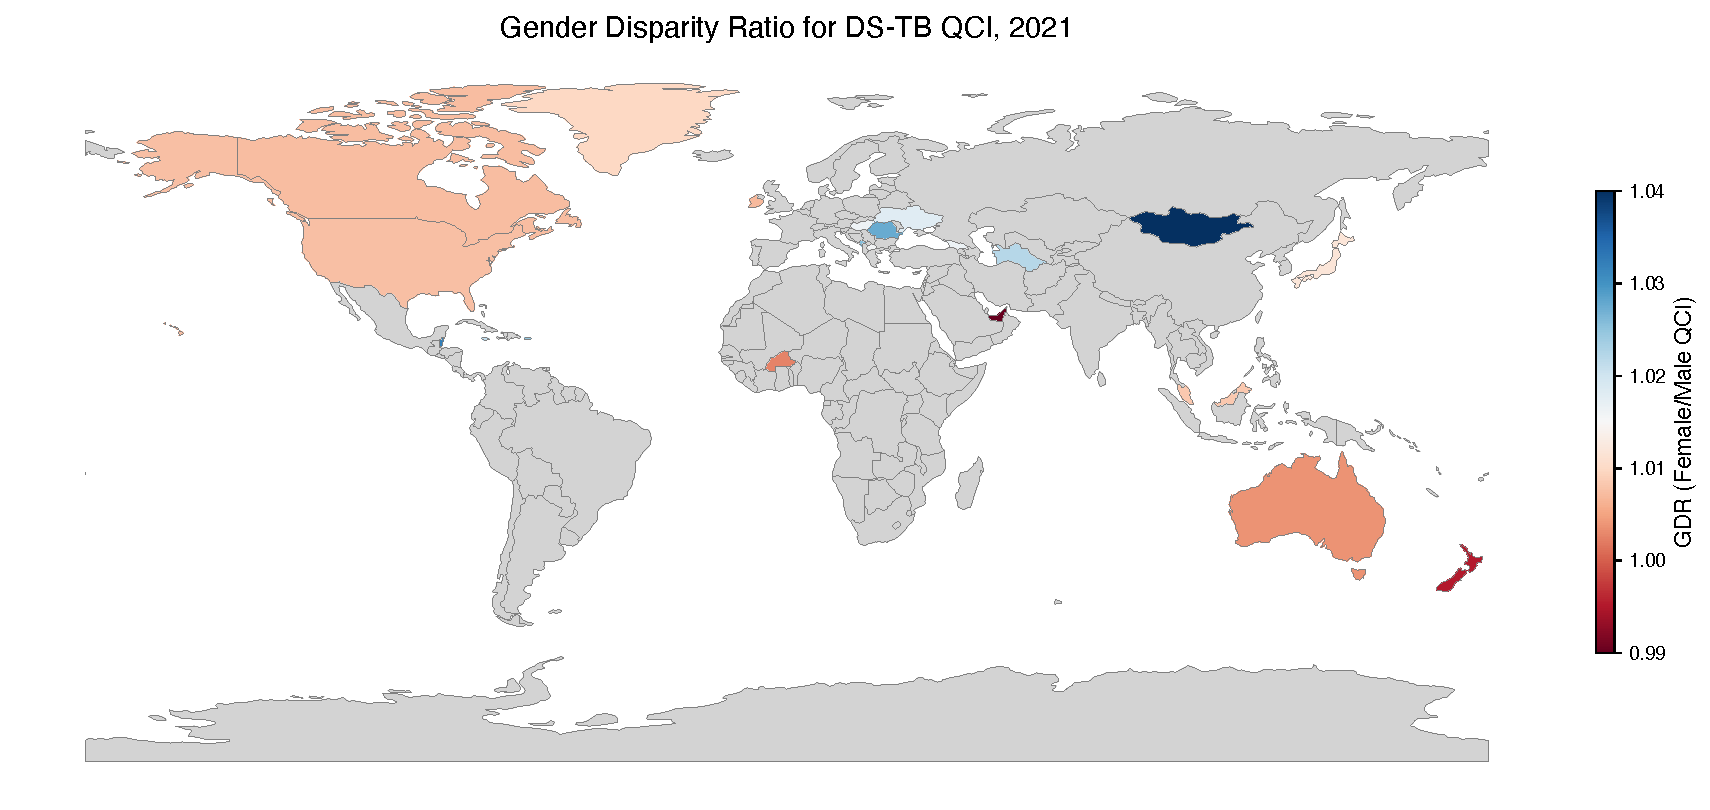
\includegraphics[width=\textwidth]{figure1_gdr_world_map.pdf}
\caption{Concentration Index of DS-TB QCI by SDI, 1990--2021. Positive values indicate pro-rich concentration. Shaded area represents 95\% confidence intervals. The CI peaked around 2000 before declining.}
\label{fig:figure1}
\end{figure}

\clearpage

\begin{figure}[htbp]
\centering

\includegraphics[width=\textwidth]{figure2_concentration_curves.pdf}
\caption{Concentration curves for DS-TB QCI ranked by SDI, 1990 and 2021. Both curves lie below the line of equality, indicating pro-rich concentration. The 2021 curve is closer to the diagonal, indicating reduced inequality.}
\label{fig:figure2}
\end{figure}

\clearpage

\begin{figure}[htbp]
\centering

\includegraphics[width=\textwidth]{figure3_inequality_indices.pdf}
\caption{Trends in inequality measures, 1990--2021. (A) Gini coefficient, (B) Generalised entropy indices (Theil T and Theil L), (C) Slope Index of Inequality with 95\% CI, (D) Relative Index of Inequality with 95\% CI.}
\label{fig:figure3}
\end{figure}

\clearpage

\begin{figure}[htbp]
\centering

\includegraphics[width=\textwidth]{figure4_gdr_sdi.pdf}
\caption{Convergence analysis. (A) Sigma-convergence: cross-country SD of QCI declining over time. (B) Beta-convergence: countries with lower baseline QCI (1990) experienced larger improvements. Points coloured by SDI group.}
\label{fig:figure4}
\end{figure}

\clearpage

\begin{figure}[htbp]
\centering
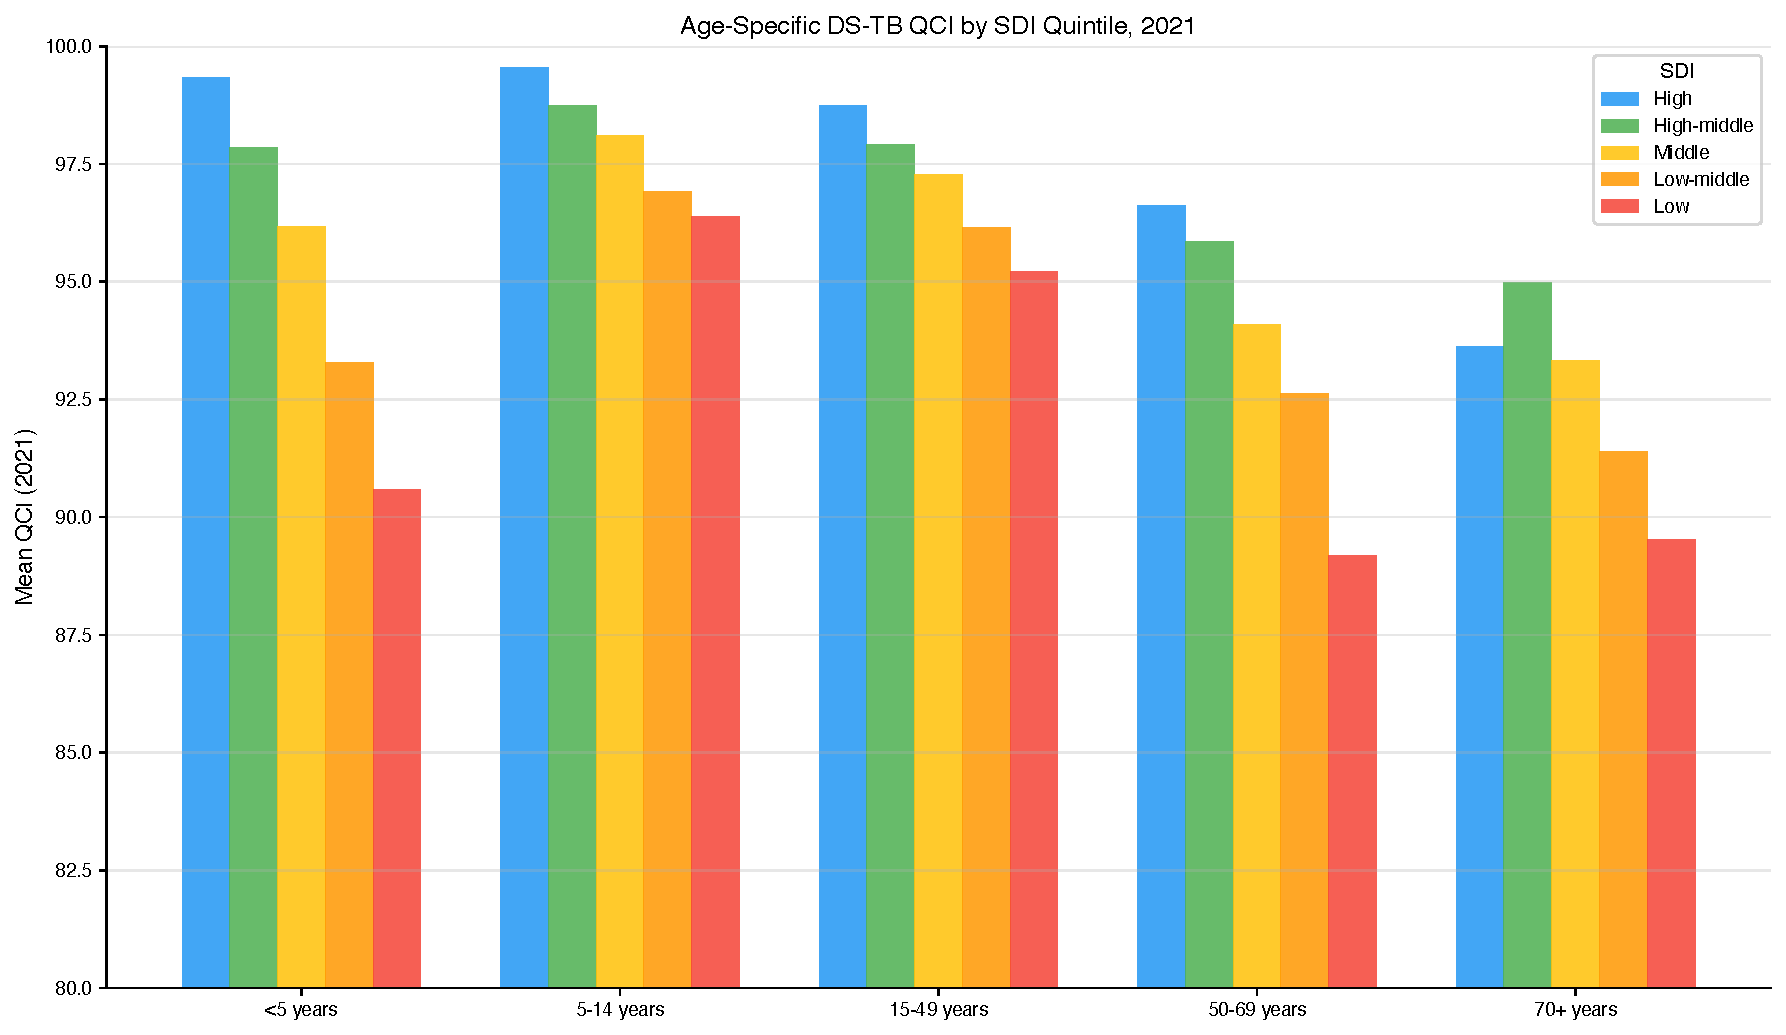
\includegraphics[width=\textwidth]{figure5_age_sdi_bars.pdf}
\caption{Gender disparity in DS-TB QCI. (A) Mean GDR over time, (B) GDR by World Bank region in 2021 (boxplot), (C) GDR versus SDI in 2021 (scatter plot with trend line).}
\label{fig:figure5}
\end{figure}

\clearpage

\begin{figure}[htbp]
\centering
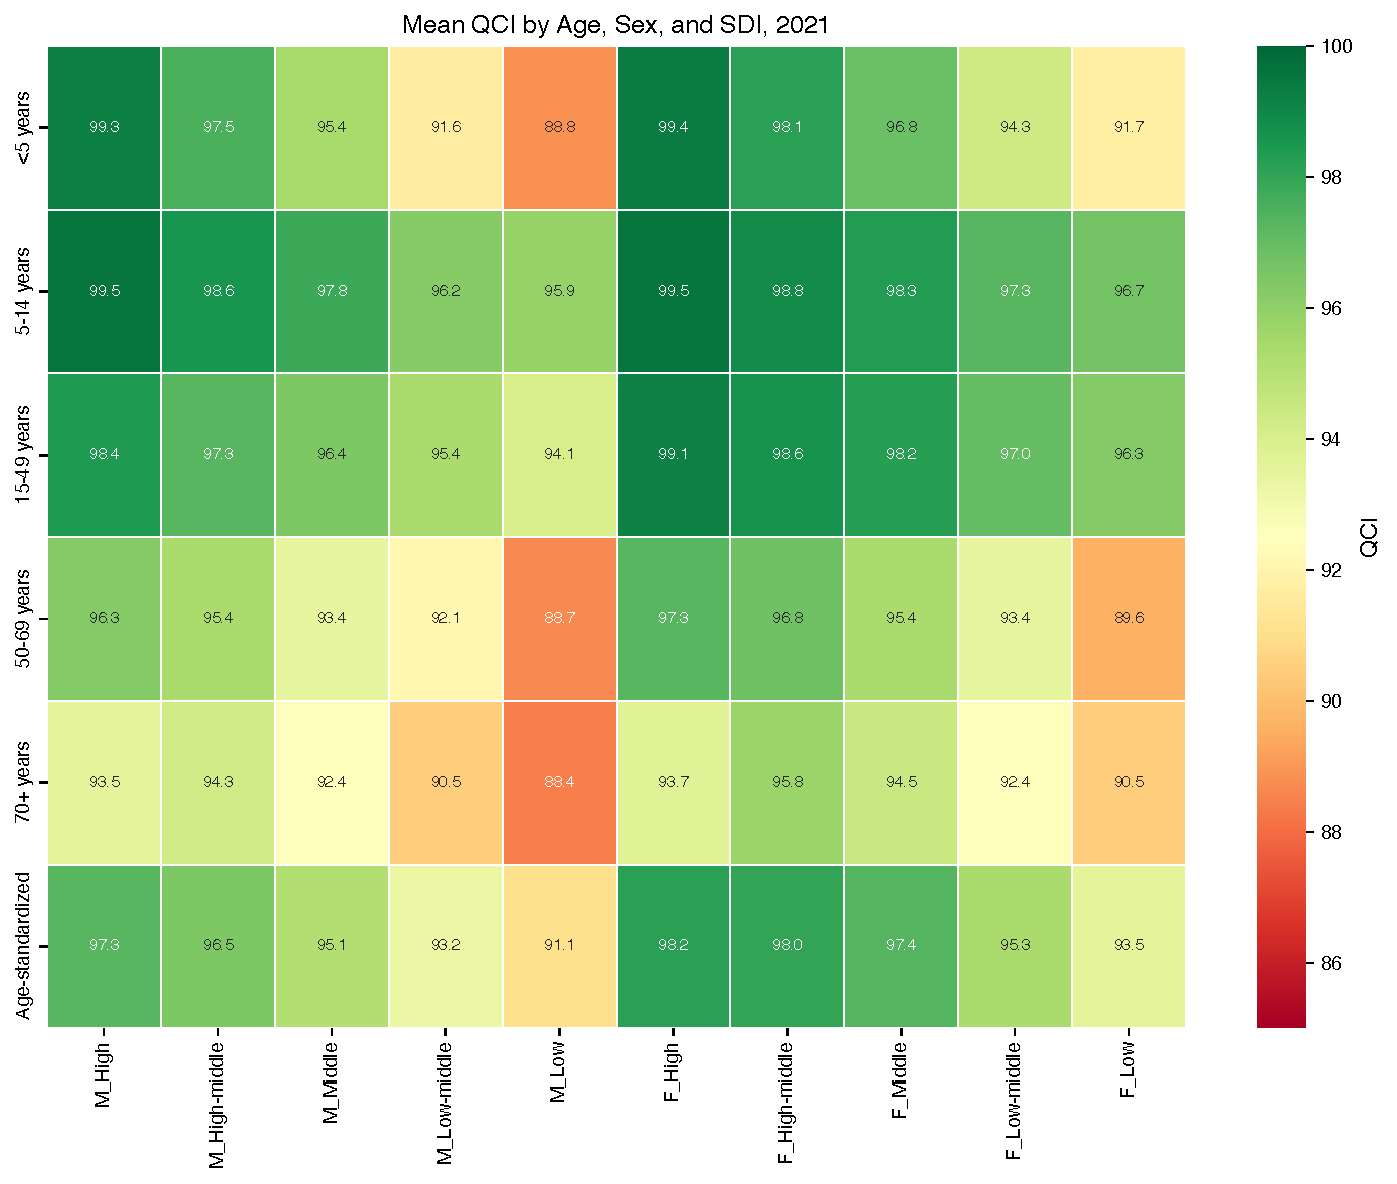
\includegraphics[width=\textwidth]{figure6_age_sex_sdi_heatmap.pdf}
\caption{Age-related inequality in DS-TB QCI. (A) Concentration Index by age group (2021), showing highest inequality for children $<$5 years. (B) Mean age-group QCI range by SDI group over time, showing declining but persistent inequality.}
\label{fig:figure6}
\end{figure}

\clearpage

\begin{figure}[htbp]
\centering

\includegraphics[width=\textwidth]{figure7_ci_by_age.pdf}
\caption{Wagstaff decomposition of the Concentration Index, 1990 and 2021. MIR (case fatality) is the dominant contributor, accounting for 40\% of wealth-related inequality.}
\label{fig:figure7}
\end{figure}

\clearpage

\begin{figure}[htbp]
\centering

\includegraphics[width=\textwidth]{figure8_female_vs_male.pdf}
\caption{Theil index decomposition: between-region versus within-region inequality, 1990--2021. The between-region share increased from 23.8\% to 34.1\%, indicating faster decline in within-region variation.}
\label{fig:figure8}
\end{figure}

%% ============================================================
%% REFERENCES
%% ============================================================

\clearpage

\begin{thebibliography}{31}

\bibitem{ref1}
World Health Organization. Global tuberculosis report 2023. Geneva: WHO; 2023.

\bibitem{ref2}
Pai M, Behr MA, Dowdy D, et al. Tuberculosis. \textit{Nat Rev Dis Primers} 2016; \textbf{2}: 16076.

\bibitem{ref3}
Kruk ME, Gage AD, Arsenault C, et al. High-quality health systems in the Sustainable Development Goals era: time for a revolution. \textit{Lancet Glob Health} 2018; \textbf{6}: e1196--252.

\bibitem{ref4}
World Health Organization. The End TB Strategy. Geneva: WHO; 2015.

\bibitem{ref5}
[Authors]. Global, Regional, and National Quality of Care Index for Drug-Susceptible Tuberculosis, 1990--2021: A Systematic Analysis of the Global Burden of Disease Study 2021. [Manuscript submitted for publication].

\bibitem{ref6}
Wagstaff A, Paci P, van Doorslaer E. On the measurement of inequalities in health. \textit{Soc Sci Med} 1991; \textbf{33}: 545--57.

\bibitem{ref7}
Mackenbach JP, Kunst AE. Measuring the magnitude of socio-economic inequalities in health: an overview of available measures illustrated with two examples from Europe. \textit{Soc Sci Med} 1997; \textbf{44}: 757--71.

\bibitem{ref8}
Barro RJ, Sala-i-Martin X. Convergence across states and regions. \textit{Brookings Papers on Economic Activity} 1991; \textbf{1}: 107--82.

\bibitem{ref9}
Sala-i-Martin X. The world distribution of income: falling poverty and convergence, period. \textit{Q J Econ} 2006; \textbf{121}: 351--97.

\bibitem{ref10}
GBD 2021 Diseases and Injuries Collaborators. Global, regional, and national incidence, prevalence, and years lived with disability for 354 diseases and injuries for 195 countries and territories, 1990--2021: a systematic analysis for the Global Burden of Disease Study 2021. \textit{Lancet} 2024; \textbf{403}: 2162--203.

\bibitem{ref11}
Kakwani N, Wagstaff A, van Doorslaer E. Socioeconomic inequalities in health: measurement, computation, and statistical inference. \textit{J Econometrics} 1997; \textbf{77}: 87--103.

\bibitem{ref12}
Atkinson AB. On the measurement of inequality. \textit{J Econ Theory} 1970; \textbf{2}: 244--63.

\bibitem{ref13}
Shorrocks AF. Decomposition procedures for distributional analysis: a unified framework based on the Shapley value. \textit{J Econ Inequality} 2013; \textbf{11}: 99--126.

\bibitem{ref14}
Wagstaff A, van Doorslaer E, Watanabe N. On decomposing the causes of health sector inequalities with an application to malnutrition inequalities in Vietnam. \textit{J Econometrics} 2003; \textbf{112}: 207--23.

\bibitem{ref15}
Stevens GA, Alkema L, Black RE, et al. Guidelines for Accurate and Transparent Health Estimates Reporting: the GATHER statement. \textit{Lancet} 2016; \textbf{388}: e19--23.

\bibitem{ref16}
GBD 2019 Demographics Collaborators. Global age-sex-specific fertility, mortality, healthy life expectancy (HALE), and population estimates in 204 countries and territories, 1950--2019. \textit{Lancet} 2020; \textbf{396}: 1160--203.

\bibitem{ref17}
Commission on Social Determinants of Health. Closing the gap in a generation: health equity through action on the social determinants of health. Geneva: WHO; 2008.

\bibitem{ref18}
Subbaraman R, Nathavitharana RR, Mayer KH, et al. Constructing care cascades for active tuberculosis: a strategy for program monitoring and identifying gaps in quality of care. \textit{PLoS Med} 2019; \textbf{16}: e1002754.

\bibitem{ref19}
Horton KC, MacPherson P, Houben RMGJ, et al. Sex differences in tuberculosis burden and notifications in low- and middle-income countries: a systematic review and meta-analysis. \textit{PLoS Med} 2016; \textbf{13}: e1002119.

\bibitem{ref20}
Nhamoyebonde S, Leslie A. Biological differences between the sexes and susceptibility to tuberculosis. \textit{J Infect Dis} 2014; \textbf{209} (suppl 3): S100--6.

\bibitem{ref21}
Kwan CK, Ernst JD. HIV and tuberculosis: a deadly human syndemic. \textit{Clin Microbiol Rev} 2011; \textbf{24}: 351--76.

\bibitem{ref22}
Dodd PJ, Yuen CM, Sismanidis C, et al. The global burden of tuberculosis mortality in children: a mathematical modelling study. \textit{Lancet Glob Health} 2017; \textbf{5}: e898--906.

\bibitem{ref23}
Global Burden of Disease Collaborative Network. Global Burden of Disease Study 2021 (GBD 2021) Results. Seattle, United States: Institute for Health Metrics and Evaluation (IHME), 2022. Available from \url{https://vizhub.healthdata.org/gbd-results/}.

\bibitem{ref24}
Horton KC, White RG, Houben RMGJ. Systematic neglect of men as a key population in tuberculosis. \textit{Tuberculosis (Edinb)} 2018; \textbf{113}: 249--53.

\bibitem{ref25}
Neyrolles O, Quintana-Murci L. Sexual inequality in tuberculosis. \textit{PLoS Med} 2009; \textbf{6}: e1000199.

\bibitem{ref26}
Zar HJ, Hanslo D, Apolles P, Swingler G, Hussey G. Induced sputum versus gastric lavage for microbiological confirmation of pulmonary tuberculosis in infants and young children: a prospective study. \textit{Lancet} 2005; \textbf{365}: 130--34.

\bibitem{ref27}
World Health Organization. Guidance for national tuberculosis programmes on the management of tuberculosis in children, 2nd edn. Geneva: WHO; 2014.

\bibitem{ref28}
Glaziou P, Floyd K, Raviglione MC. Global epidemiology of tuberculosis. \textit{Semin Respir Crit Care Med} 2018; \textbf{39}: 271--85.

\bibitem{ref29}
Rajagopalan S. Tuberculosis and aging: a global health problem. \textit{Clin Infect Dis} 2001; \textbf{33}: 1034--39.

\bibitem{ref30}
GBD 2019 Healthcare Access and Quality Collaborators. Assessing performance of the Healthcare Access and Quality Index, overall and by select age groups, for 204 countries and territories, 1990--2019: a systematic analysis from the Global Burden of Disease Study 2019. \textit{Lancet Glob Health} 2022; \textbf{10}: e1715--43.

\bibitem{ref31}
Kranzer K, Afnan-Holmes H, Tomlin K, et al. The benefits to communities and individuals of screening for active tuberculosis disease: a systematic review. \textit{Int J Tuberc Lung Dis} 2013; \textbf{17}: 432--46.

\end{thebibliography}

%% ============================================================
%% END MATTER
%% ============================================================

\clearpage

\section*{Declaration of interests}

We declare no competing interests.

\section*{Data sharing}

All input data used in this study are publicly available through the GBD Results Tool (\url{https://vizhub.healthdata.org/gbd-results/}).\textsuperscript{23} The analytical code used to construct the inequality metrics, decomposition analyses, convergence tests, and all visualisations will be made available in a public repository upon publication. [Add repository URL, e.g., GitHub or Zenodo DOI.]

\section*{Contributors}

[To be completed using CRediT taxonomy -- e.g., Conceptualisation, Data curation, Formal analysis, Methodology, Visualisation, Writing (original draft), Writing (review and editing), Supervision. All authors should review and approve the final manuscript.]

\section*{GATHER compliance}

This study was conducted in accordance with the Guidelines for Accurate and Transparent Health Estimates Reporting (GATHER) and the RECORD guidelines for equity-focused analyses. A completed GATHER checklist is provided in the Supplementary Materials.

\section*{Ethical approval}

Ethical approval was not required for this study as it exclusively used publicly available, de-identified, aggregate data from the GBD 2021 Study.

\end{document}
